\documentclass[runningheads]{llncs}
\usepackage[T1]{fontenc}
\usepackage[utf8]{inputenc}
\usepackage{graphicx}
\usepackage{booktabs}
\usepackage{tabularx}
\usepackage{multirow}
\usepackage{amsmath}
\usepackage{amssymb}
\usepackage{xcolor}
\usepackage{url}
\usepackage{hyperref}
\begin{document}
\title{From Comment Generation to Review Systems: A Survey of LLM-Based Code Review (2023--2026)}
\titlerunning{A Survey of LLM-Based Code Review}
\author{Anonymous Author(s)}
\authorrunning{Anonymous}
\institute{Anonymous Institution}
\maketitle
\begin{abstract}
Between 2023 and 2026, research on code review with large language models (LLMs) moved from generating comments for mined code hunks, scored with text-similarity metrics, to multi-stage systems that run on real pull requests and are judged by issue-level precision and recall or by developer behaviour. We survey this period through a structured, multi-source literature review and argue that progress has shifted from the model to the pipeline around it: generating plausible comments is no longer the hard part, while precision, context selection and evaluation validity are. We contribute a taxonomy of seven dimensions that adds deployment cost and trust risk to the usual task view, a quantitative synthesis in which every number carries its metric name, and an agenda of twelve prioritised open gaps. The evidence shows that realistic benchmarks expose low absolute capability, that deployed systems converge on generating broadly and filtering hard, that every filter studied costs recall, that acceptance metrics are not comparable across studies, and that review-specific cost evidence is almost absent. We therefore propose treating LLM code review as a system design and measurement problem with a cost axis.
\end{abstract}
\keywords{Code review \and Large language models \and Software engineering \and Survey \and Benchmarks \and Agentic systems}
\section{Introduction}\label{sec:intro}
Code review is a central quality practice in software development, and automating parts of it has been studied for years. Between 2023 and 2026 the field changed character. Early work generated review comments for mined code hunks and scored them with BLEU-style similarity to the human comment~\cite{li2022codereviewer}. Current work builds multi-stage systems that run on real pull requests (PRs) and are judged by issue-level precision and recall, or by what developers do with the comments.

The main result of this period is that generating plausible comments is no longer the hard part. Precision, context selection and evaluation validity are. On a realistic PR-level benchmark such as SWR-Bench, the best systems still reach an F1 of only about 19--22\%~\cite{zeng2025swrbench}. In production, industrial systems converge on one design, generating broadly and then filtering hard, and the verifier that implements the filter lifted BitsAI-CR's precision from about 25\% to 75\%~\cite{sun2025bitsai}. Suppression rules took Google's AutoCommenter from 54\% to 80\% useful comments~\cite{vijayvergiya2024ai}. At the same time the attack surface is real: LLM-refined PR framing got vulnerabilities past two production reviewers in 32 of 33 cases~\cite{alexopoulos2026when}.

\textbf{Thesis.} Progress in this period moved from the model to the pipeline around it. LLM code review should be treated as a system design and measurement problem with a cost axis, not as a comment-generation task.

\textbf{Contributions.} This survey makes four contributions.
\begin{enumerate}
\item A survey of LLM-based code review for 2023--2026, built with a structured multi-source review (Section~\ref{sec:method}).
\item A taxonomy of seven dimensions that adds deployment cost (D6) and trust risk (D7) to the task, adaptation, architecture, context and evaluation dimensions used before (Section~\ref{sec:taxonomy}).
\item A quantitative synthesis in which every number names its metric and acceptance figures are explicitly marked as non-comparable (Sections~\ref{sec:benchmarks}--\ref{sec:security}).
\item An agenda of twelve prioritised open gaps (Section~\ref{sec:gaps}).
\end{enumerate}

\textbf{Organisation.} Section~\ref{sec:background} gives background and compares existing surveys, and Section~\ref{sec:method} describes the method. Sections~\ref{sec:taxonomy}--\ref{sec:security} cover the taxonomy, benchmarks, techniques, systems, deployment and security. Section~\ref{sec:gaps} lists the gaps, Section~\ref{sec:threats} discusses threats to validity, and Section~\ref{sec:conclusion} concludes.

\section{Background and Related Surveys}\label{sec:background}
\textbf{Modern code review and its tasks.} Modern code review is the lightweight, tool-supported inspection of a change before it is merged. Work on automating it covers many tasks. The dedicated systematic review of automating code review covers 119 studies across 34 tasks in 9 macro-categories, and reviewer recommendation dominates it with 36 papers~\cite{tufano2025automating}. Three tasks matter most for LLMs: generating review comments, detecting issues in a change, and refining code according to a comment.

\textbf{Pre-LLM baselines.} Pre-trained models set the baselines that later work compares against. Tufano et al. showed that pre-trained models boost code review automation~\cite{tufano2022using}, and CodeReviewer pre-trained on large-scale review data and became the standard foundational model and dataset~\cite{li2022codereviewer}. Evaluation at that stage relied on similarity to the human reference comment.

\textbf{Existing surveys.} Table~\ref{tab:surveys} compares the surveys we found. Only one systematic review is dedicated to automating code review, and its search ran until 20 December 2024~\cite{tufano2025automating}. It names cost as a barrier in only 5 papers. Broader reviews of modern code review~\cite{yang2025roadmap,badampudi2023modern,davila2021systematic} and the general LLM4SE surveys~\cite{hou2023large,zhang2023survey,fan2023large} treat review as one topic among many. Khan et al. cover only benchmarks and evaluation~\cite{khan2026survey}, and the only efficiency-focused LLM4SE review is not specific to review~\cite{shi2024efficient}. We found no survey dedicated to LLM-based or agentic code review over 2024--2026 that systematically covers cost, small models, cascades or learning from feedback. This absence is likely but not certain, because our coverage of 2026 journals is incomplete.

\begin{table}[t]
\caption{Existing surveys relevant to LLM-based code review. Counts are as reported by each survey; a dash means no count was recorded.}\label{tab:surveys}
\setlength{\tabcolsep}{3pt}
\small
\begin{tabularx}{\textwidth}{@{}p{2.6cm}p{2.5cm}p{1.3cm}Xcc@{}}
\toprule
Survey & Period & Studies & Focus & Cost & Agents \\
\midrule
Tufano \& Bavota~\cite{tufano2025automating} & search to Dec. 2024 & 119 & Automating code review (34 tasks) & partly & no \\
Yang et al.~\cite{yang2025roadmap} & 2013--2025 & 231 (v1) & Modern code review, broad & no & no \\
Khan et al.~\cite{khan2026survey} & pre-LLM and LLM era & 99 & Benchmarks and evaluation only & no & no \\
Badampudi et al.~\cite{badampudi2023modern} & up to 2021 & 244 & Modern code review (pre-LLM) & no & no \\
Davila \& Nunes~\cite{davila2021systematic} & pre-LLM & --- & Taxonomy of modern code review & no & no \\
Hou et al.~\cite{hou2023large} & LLM4SE & 395 & LLMs for SE; review is one task & no & no \\
Zhang et al.~\cite{zhang2023survey} & LLM4SE & 947 & LLMs for SE; review is one task & no & no \\
Fan et al.~\cite{fan2023large} & LLM4SE & --- & LLMs for SE, open problems & no & no \\
Shi et al.~\cite{shi2024efficient} & LLM4SE & --- & Efficient and green LLM4SE & general & no \\
\bottomrule
\end{tabularx}
\end{table}

\section{Review Method}\label{sec:method}
This survey is a structured, multi-source literature review. It is not a full systematic literature review following PRISMA, and we do not report counts of screened or excluded papers.

\textbf{Sources and period.} We searched arXiv, the ACM Digital Library, IEEE Xplore, DBLP and Semantic Scholar for work from 2023 to 2026, together with pre-2023 baselines and earlier surveys needed for context. The consolidated corpus contains 139 works.

\textbf{Inclusion and exclusion.} We included studies on LLM-based or LLM-adjacent code review: comment generation, issue detection, refinement, comment classification, security review, static-analysis triage, benchmarks, deployments and human studies. We also included general work on cascades, routing and distillation when it bears on cost, and marked it as not review-specific. We excluded two systems named in our initial brief because we could not locate them in arXiv or Semantic Scholar, and we did not cite grey literature as evidence.

\textbf{Verification.} Metadata was checked on 11 November 2026 against primary sources: arXiv abstract pages, the arXiv and Semantic Scholar APIs, the ACL Anthology, PMLR, Crossref and conference pages. Where a venue could not be confirmed we cite the work as an arXiv preprint.

\textbf{Extraction.} For each work we extracted attributes along the seven dimensions of the taxonomy in Section~\ref{sec:taxonomy}, together with reported metrics, each stored with its metric name. Most numbers come from abstracts or arXiv HTML full texts, and figures that came only from search snippets were dropped or labelled.

\section{A Taxonomy of LLM-Based Code Review}\label{sec:taxonomy}

Existing taxonomies are organised by task: 34 tasks in nine macro-categories~\cite{tufano2025automating}, or five domains and 18 tasks for benchmarks~\cite{khan2026survey}. None captures the system-level, cost and risk dimensions that dominate 2024--2026 work. We therefore classify each work on seven orthogonal dimensions, so that a paper occupies one cell per dimension (Fig.~\ref{fig:taxonomy}).

\begin{itemize}
\item \textbf{D1 Review task:} necessity estimation, comment generation, issue detection in PRs, refinement, comment classification, security review, static-analysis warning triage, multi-round review, and evaluation.
\item \textbf{D2 Model adaptation:} pre-training, full fine-tuning, PEFT, prompting, RAG, preference/RL, reasoning tuning, data-centric methods, and distillation.
\item \textbf{D3 System architecture:} single call, generator plus filter, multi-role agents, tool-using agents, static-analysis hybrids, multi-run aggregation, and routing.
\item \textbf{D4 Context scope:} hunk, function, file, repository, and non-code intent.
\item \textbf{D5 Evaluation regime:} text similarity, LLM judges, issue-level precision/recall, comprehension probes, tests, field outcomes, and controlled experiments.
\item \textbf{D6 Deployment and cost profile (new):} frontier API, self-hosted large model, small or local model, cascade or routing, and whether tokens, dollars or latency are reported.
\item \textbf{D7 Trust and risk treatment (new):} false-positive control, hallucination detection, adversarial robustness, human factors, and privacy.
\end{itemize}

D6 and D7 are the main additions. Cost and risk are already visible in the evidence: one industrial study reports a cost of about \$0.48 per PR together with a longer PR closure time~\cite{cihan2025automated}, hallucination detection has its own industrial method~\cite{tantithamthavorn2026hallujudge}, and attacks on real review pipelines~\cite{alexopoulos2026when,isbarov2026gitinject} and anchoring in a controlled experiment~\cite{tufano2025deep} are now documented.

Mapped onto this grid, the literature piles up in one region: comment generation or issue detection (D1), PEFT or prompting (D2), a single call or generator-plus-filter pipeline (D3), issue-level or field evaluation (D5), and frontier APIs (D6). Two regions are essentially empty: small or cascaded models evaluated on real-PR issue detection (D6 crossed with D5), and defences against adversarial attacks (D7), as opposed to the attacks themselves.

\begin{figure}[t]
\centering
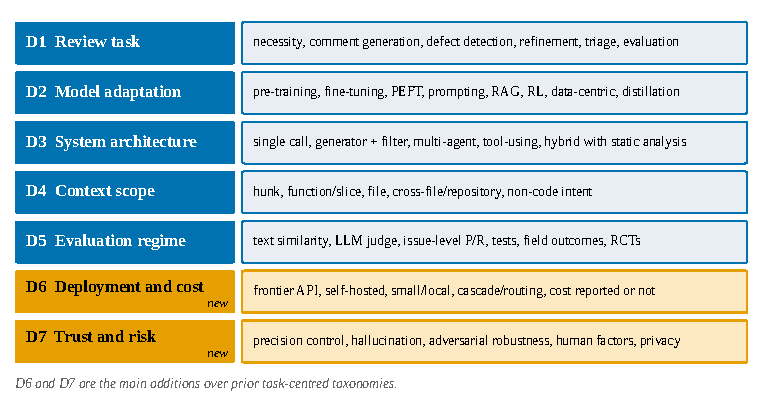
\includegraphics[width=\textwidth]{figures/taxonomy.pdf}
\caption{Proposed taxonomy: seven orthogonal dimensions (D1 review task, D2 model adaptation, D3 system architecture, D4 context scope, D5 evaluation regime, D6 deployment and cost profile, D7 trust and risk treatment) with their summarised categories. D6 and D7 are highlighted as additions over prior task-oriented taxonomies.}
\label{fig:taxonomy}
\end{figure}

\section{Benchmarks and Evaluation}\label{sec:benchmarks}

\paragraph{Foundational datasets.} Tufano et al.\ automated two review activities, implementing a reviewer's comment in up to 31\% of cases~\cite{tufano2021towards}. CodeReviewer defined the three tasks later reused (quality estimation, comment generation, refinement) on 1,161 GitHub repositories in nine languages, with baselines of QE F1 71.53, comment-generation BLEU-4 5.32 and refinement BLEU 82.61~\cite{li2022automating}. These datasets fixed diff-only inputs, a single reference per change and text-similarity scoring.

\paragraph{Text similarity fails.} Against human relevance judgements, BLEU reaches Kendall $\tau=0.001$ and chrF++ $\tau=0.1555$, whereas reference-free CRScore reaches $\tau=0.4567$~\cite{naik2025crscore}. A ``copy the input'' baseline scores refinement BLEU 58.75 with 0\% exact match~\cite{li2022automating}. DeepCRCEval found that a BLEU-optimised CodeReviewer scored 1.77 on actionability (1--10 scale), against about 9.4--10 for a few-shot GPT-4 reviewer~\cite{lu2025deepcrceval}.

\paragraph{Noisy ground truth.} TooNoisy found 36\% noisy comments in a 270-comment training sample~\cite{liu2025toonoisy}, and DeepCRCEval judged only 3\% (Tufano) and 8\% (CodeReviewer) of sampled references ``ideal''~\cite{lu2025deepcrceval}. Noise also runs the other way: expert verification added 1,114 issues to 391 original PR comments (+285\%) in AACR-Bench, so a model finding a real but uncommented issue is scored as a false positive~\cite{zhang2026aacr}.

\paragraph{PR-level benchmarks, low scores.} The 2025--2026 benchmarks use hundreds of verified PRs with repository context and score issue detection (Fig.~\ref{fig:benchmarks}b). Best results are modest: F1 19.38\% on SWR-Bench, rising to 21.91\% with ten aggregated runs~\cite{zeng2025swr}; F1 16.12\% on AACR-Bench, where the highest recall of 47.24\% came at 6.70\% precision~\cite{zhang2026aacr}; 15--31\% of human-flagged issues detected on SWE-PRBench~\cite{kumar2026swe}; about 33\% known-defect detection rate on CR-Bench-v2~\cite{pereira2026crbenchv2}; and a 32.1\% test pass rate for Claude Code on c-CRAB~\cite{zhang2026ccrab}. Most of these are unreviewed arXiv preprints. Synthetic data overstates capability (Fig.~\ref{fig:benchmarks}a): one study reports F1 0.847 on mutation-injected samples against 0.066 on real PRs~\cite{kumar2026bigger}, and a 7B model fell from 68.26\% F1 on BigVul to 3.09\% on PrimeVul~\cite{ding2025vulnerability}.

\paragraph{Unvalidated, incomparable judges.} LLM-as-judge is now the de facto scorer, but validation is thin and judges differ across benchmarks. SWR-Bench validated its judge on 100 reports~\cite{zeng2025swr}, SWE-PRBench reports $\kappa=0.75$ against humans~\cite{kumar2026swe}, and AACR-Bench uses a different judge model~\cite{zhang2026aacr}. No leaderboard runs the same models across benchmarks, so metrics and rankings are not comparable.

\begin{figure}[t]
\centering
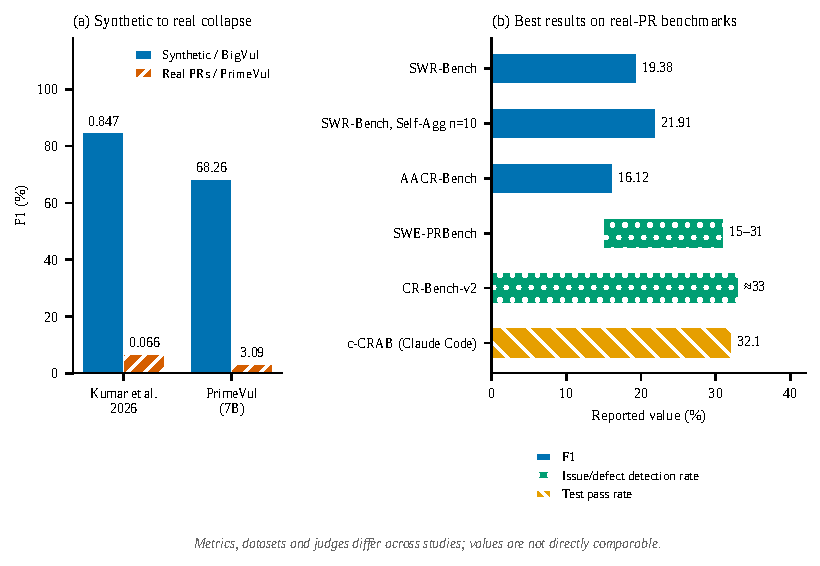
\includegraphics[width=\textwidth]{figures/benchmarks.pdf}
\caption{(a) Collapse from synthetic to real data: F1 0.847 on mutation-injected samples versus 0.066 on real PRs~\cite{kumar2026bigger}, and 7B-model F1 of 68.26\% on BigVul versus 3.09\% on PrimeVul~\cite{ding2025vulnerability}. (b) Best reported results on real-PR benchmarks, each bar labelled with its own metric: SWR-Bench F1 19.38\% (21.91\% with Self-Agg, $n=10$), AACR-Bench F1 16.12\%, SWE-PRBench 15--31\% of issues detected (interval), CR-Bench-v2 about 33\% known-defect detection, and c-CRAB 32.1\% test pass rate (Claude Code). Metrics differ and are not comparable.}
\label{fig:benchmarks}
\end{figure}

\section{Model-Level Techniques}\label{sec:techniques}

\textbf{Parameter-efficient fine-tuning.} LLaMA-Reviewer fine-tuned LLaMA-6.7B with LoRA, training under 1\% of the parameters, and reached RCG BLEU-4 of 5.70 against 5.32 for CodeReviewer, with QE F1 of 70.49 against 71.53 \cite{lu2023llamareviewer}. We found no head-to-head comparison of full fine-tuning and LoRA for review. Under cold start, few-shot prompting beat zero-shot by 46.38--659.09\% relative exact match (EM), and the authors advise few-shot prompting without a persona; fine-tuned GPT-3.5 gained 73.17--74.23\% EM over a prompting baseline \cite{pornprasit2024finetuning}.

\textbf{Retrieval.} Retrieval is helpful but not monotone. RARe reached BLEU-4 of 12.32 and 12.96 and found top-1 retrieval best, because further exemplars added redundancy and conflicting cues \cite{meng2025retrieval}. LAURA, which combines exemplar retrieval, context augmentation and guidance, obtained a human ``completely correct or at least helpful'' rate of 42.2\% with GPT-4o and 40.4\% with the open-weight DeepSeek-V3 \cite{zhang2025laura}.

\textbf{Data-centric curation.} Data quality repeatedly matters more than size. Training on LLM-filtered data raised BLEU-4 by 7.5--13.0\% and human informativeness from 3.44 to 4.27 (1--5 scale), whereas size-matched random subsets gave no gain \cite{liu2025noisy}. Desiview identified desired comments in over 150K CodeReviewer entries at F1 of 84.44\% and added KTO alignment using undesired comments as negatives, which slightly beat plain fine-tuning \cite{yu2024distilling}. Supervised fine-tuning on raw CodeReviewer human reviews did far worse than zero-shot, with 3B Python comprehensiveness (LLM judge, 0--1) falling to 0.10 \cite{kapadnis2025crscore}.

\textbf{Reinforcement and preference optimisation.} CoRAL applies PPO with a reward based on semantic similarity or on a refinement model implementing the comment, reaching median BLEU of 8.67 against 7.05 for SFT alone; its o3-mini judge was validated on only 100 pairs \cite{sghaier2025leveraging}. CRScore++ adds DPO on tool-grounded demonstrations and raised 3B Python comprehensiveness from 0.43 to 0.67 \cite{kapadnis2025crscore}. MelcotCR uses long chain-of-thought tuning, and a 14B Qwen2.5 became on par with the 671B DeepSeek-R1 at detecting and describing issues \cite{yu2025finetuning}. Every reward in these papers is an LLM judge, an embedding similarity or a BLEU-family score, and no large human study has confirmed the gains.

\textbf{Open versus proprietary models.} Meta's fine-tuned Llama beat GPT-4o by 9 points of exact match (68\%) on comment-to-patch, and by 9.2 points in the production ActionableToApplied rate (19.7\%) \cite{maddila2025aiassisted}. The pattern is that prompted proprietary models suit cold start, while fine-tuned open models compete once in-domain data exist.

\textbf{Comment-quality classification.} LLMs beat a trained deep-learning classifier across 17 fine-grained comment categories, especially for rare useful ones \cite{nguyen2025exploring}, so classifiers can now serve as data filters and as reward signals.

\textbf{Caveat on BLEU.} The BLEU values above are not comparable across papers: variants differ (BLEU-4, median BLEU, trimmed BLEU), test sets differ, and BLEU itself barely tracks human judgement (Kendall $\tau$ of 0.001 against human relevance, versus 0.4567 for the reference-free CRScore) \cite{naik2025crscore}.

\section{System Architectures}\label{sec:systems}

\textbf{Generate broadly, filter hard.} The industrial systems we found share one shape, shown in Fig.~\ref{fig:pipeline}: a context builder feeds a generator, and one or more explicit precision gates follow before comments reach developers. Examples are BitsAI-CR's ReviewFilter \cite{sun2025bitsai}, RovoDev's LLM judge plus a learned gate \cite{tantithamthavorn2026rovodev}, AutoCommenter's confidence thresholds \cite{vijayvergiya2024aiassisted}, and the Meta-Reviewer and Validator stages of the ICML 2025 pipeline \cite{lu2025towards}. Free-form multi-agent conversation appeared in no industrial report.

\begin{figure}[t]
\centering
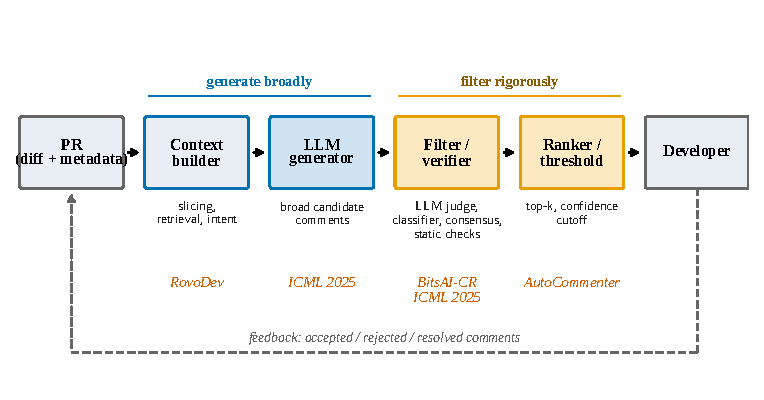
\includegraphics[width=\linewidth]{figures/pipeline.pdf}
\caption{The ``generate broadly, filter hard'' pipeline, with example systems under each stage.}
\label{fig:pipeline}
\end{figure}

\textbf{Architecture families.} The literature contains nine recurring designs, including fine-tuned detector plus verifier, multi-role pipelines with slicing and validation, a single context-aware call with judge and gate, bounded-tool agents, LLM plus static analysis, mixture of prompts, threshold-based prediction and multi-run aggregation.

\textbf{Purpose-built versus general agents.} On AACR-Bench, Claude Code produced only about 0.09--0.15 comments per patch, with high precision and low recall \cite{zhang2026aacrbench}. OpenCodeReview, an unrefereed preprint, reports SEM-F1 of 25.10\% against 11.57\% for the same Claude-4.6-Opus model inside Claude Code, using 5--15$\times$ fewer tokens \cite{li2026opencodereview}. The authors are largely Alibaba-affiliated and evaluate on an Alibaba-built benchmark.

\textbf{Selective versus exhaustive context.} More context is not automatically better. On AACR-Bench, adding top-3 BM25 contexts dropped Claude's F1 from 14.46 to 9.98 \cite{zhang2026aacrbench}. On SWE-PRBench, a 2,000-token diff-plus-summary prompt beat a 2,500-token full-context prompt for every model \cite{kumar2026swe}. What is chosen seems to matter more than how much, but no controlled, cost-reporting ablation exists.

\textbf{Verifiers always cost recall.} BitsAI-CR's ReviewFilter moved offline precision/recall from 57.03/45.50 to 65.59/39.77 \cite{sun2025bitsai}, and the ICML authors note that self-correction can discard critical bug-detecting comments \cite{lu2025towards}. Independence helps: Claude reviewing Codex drafts raised the pass rate from 71.6\% to 89.7\%, Codex reviewing Claude drafts lowered it from 91.4\% to 82.8\%, and Claude's self-review changed nothing \cite{xiang2026crossmodel}. Consensus is not truth: ten dedicated reviewers unanimously endorsed a non-existent OpenSSL padding oracle, and only an empirical test killed it \cite{agarwal2026refute}.

\textbf{Static-analysis triage.} When the LLM adjudicates one bounded question about a single warning, results are strong. At Tencent, hybrid LLM and static-analysis techniques removed 94--98\% of false positives while maintaining high recall, at \$0.0011--\$0.12 per alarm \cite{du2026reducing}. The lesson is to give the LLM narrowly scoped adjudication tasks and leave candidate generation to deterministic analysers where possible.

\section{Industrial Deployments and Human Factors}\label{sec:deployment}

Production reports share one caveat: every firm defines ``success'' differently, so the headline numbers in Fig.~\ref{fig:field} measure different things and must not be ranked against each other.

\textbf{Industrial deployments.}
Google's AutoCommenter reports a comment-resolution rate of about 40\%, and 80\% of raw comments would have landed on unmodified lines before filtering. A large A/B test with about half of Google's developers showed no significant change in review duration~\cite{vijayvergiya2024ai}.
ByteDance's BitsAI-CR reports an Outdated Rate (share of flagged lines later modified) of 26.7\% for Go against 35--46\% for human comments; second-week retention was 61.64\%~\cite{sun2025bitsai}.
At Atlassian, RovoDev's code-resolution rate was 38.70\% against 44.45\% for human comments, and median PR cycle time fell 30.8\% (observational, not randomised)~\cite{tantithamthavorn2026rovodev}.
Meta's fine-tuned model reached a 19.7\% ActionableToApplied rate, the share of suggested patches that authors apply~\cite{maddila2025ai}.
At Beko, 73.8\% of PR-Agent comments were marked ``Resolved'', but resolution is a mandatory label set before merge, and average PR closure time rose from 5h52m to 8h20m~\cite{cihan2025automated}. A follow-up found that LLM-judge agreement with engineers' labels was only 0.44--0.62~\cite{karakaya2026understanding}.
At Mozilla and Ubisoft, reviewers accepted 8.1\% and 7.2\% of RevMate's comments~\cite{olewicki2024impact}.
Ericsson has reported only an experience report and an offline validation of a multi-agent reviewer (96\% of more than 200 flagged issues validated), not field acceptance rates~\cite{ramesh2025automated}.

\begin{figure}[t]
\centering
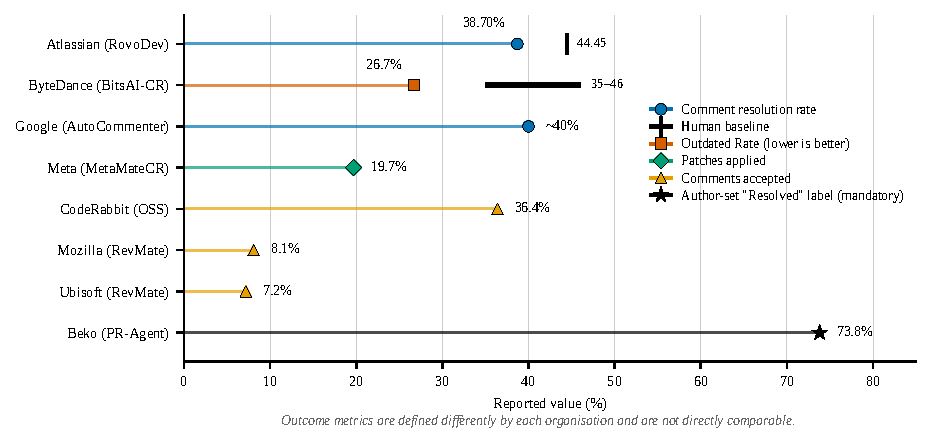
\includegraphics[width=\linewidth]{figures/field_outcomes.pdf}
\caption{Field outcomes by organisation, with the human baseline where one was measured. Markers differ by metric type; the values are not comparable across studies.}
\label{fig:field}
\end{figure}

\textbf{Open-source mining.}
In 31,073 CodeRabbit review/feedback pairs, 36.4\% were accepted and 56.3\% rejected, mainly as false positives and redundancy~\cite{lin2026agentic}.

\textbf{Controlled evidence.}
In the one controlled experiment (29 experts), reviewers given an LLM review concentrated on the flagged locations and found more low-severity but not more high-severity issues, with no time saved: an anchoring effect~\cite{tufano2025deep}.
The evidence on cycle time conflicts: Atlassian observed a reduction, Beko an increase, and Google no significant change.
The only randomised trial, at Meta, found that showing AI patches to reviewers slowed reviews by more than 5\%, while showing them only to authors removed the regression~\cite{maddila2025ai}.

\textbf{Human and organisational factors.}
Interviewees reported that cognitive load sometimes rises because of the LLM's excessive details~\cite{alami2025human}. Atlassian's 35.6\% drop in human comments per PR raises an open question: do workload savings come from displacing human scrutiny? Privacy is handled mainly by design: Google, Meta and ByteDance run in-house models, whereas Beko and Mozilla/Ubisoft used third-party APIs~\cite{sun2025bitsai,cihan2025automated,olewicki2024impact}.

\section{Security and Reliability}\label{sec:security}

\textbf{LLMs versus SAST.}
Across 7 LLMs and 5 prompts, LLMs significantly outperformed SAST tools on security code review~\cite{yu2024insight}. At repository level, 12 open LLMs detected 90--100\% of vulnerabilities but with many false positives, whereas 15 SAST tools had low detection and few false positives; ensembling partly offsets both weaknesses~\cite{zhou2024comparison}.
Realistic data changes the picture: a 7B model scoring 68.26\% F1 on BigVul scored 3.09\% on PrimeVul~\cite{ding2025vulnerability}.

\textbf{Hallucination and unfaithful reasoning.}
Every deployment reports ungrounded comments, yet the notes found no peer-reviewed per-comment hallucination rate for a production reviewer. Atlassian's HalluJudge detects context-misaligned hallucinations at F1 0.85 for about \$0.009 per assessment, but its abstract gives no base rate~\cite{tantithamthavorn2026hallujudge}. Accuracy-only metrics also miss correct verdicts reached through wrong reasoning, which are acknowledged but not quantified in the review setting.

\textbf{Attacks.}
Three attack families succeed against real pipelines. Templated bias in PR metadata was ineffective, but LLM-refined PR framing reintroduced the vulnerability past Claude Code and CodeRabbit in 32 of 33 cases~\cite{alexopoulos2026when}. Flashboom decoy code blinded auditors with success up to 96.3\% on CodeLlama and 83.05\% on Gemma~\cite{li2025make}. GitInject ran 11 scenarios against five live GitHub Actions workflows from four AI providers; every provider fell to at least one high-severity injection, because configuration files from unmerged contributions are loaded as operator-level instructions~\cite{isbarov2026gitinject}.
The evidence is not uniform: in-code adversarial comments were not significantly effective against eight frontier detectors over 9,366 trials~\cite{thornton2026can}. The gap plausibly reflects channel and optimisation (iterative versus templated); we read both as showing that naive manipulation is weak and optimised manipulation is not. Several of these results are 2026 preprints.

\textbf{Mitigations.}
In the same study, SAST cross-referencing was the best defence (96.9\% detection), while stripping comments hurt weaker models~\cite{thornton2026can}. LLM triage of SAST warnings is promising: at Tencent, hybrid techniques removed 94--98\% of false positives while maintaining high recall~\cite{du2026reducing}, and QASecClaw raised F1 from 78.39\% (Semgrep alone) to 90.93\% at a 3.1\% recall cost (preprint)~\cite{ameen2026qasecclaw}.

\textbf{Non-determinism.}
We found no review-specific measurement of output variance; the only evidence comes from code generation, where we did not cite it, so repeated-run reporting remains a gap.

\section{Open Challenges and Research Agenda}\label{sec:gaps}

The evidence reviewed above leaves twelve gaps, ordered by how strongly the evidence demands them, how many independent sources raise them, and how directly a low-cost architecture can address them. Table~\ref{tab:gaps} summarizes them. Most are cost, evaluation or deployment questions rather than questions about the generator.

\begin{table}[t]
\centering
\caption{Twelve prioritized open gaps. Metrics are not comparable across studies.}
\label{tab:gaps}
\footnotesize
\begin{tabularx}{\textwidth}{@{}r>{\raggedright\arraybackslash}p{2.6cm}>{\raggedright\arraybackslash}X>{\raggedright\arraybackslash}X@{}}
\toprule
\# & Gap & Key evidence & Research direction \\
\midrule
1 & Cost--quality trade-offs & General cascades save 40--98\% of cost~\cite{chen2023frugalgpt}, a code-completion cascade 26--70\%~\cite{chen2024model}; no review cascade evaluated, and no industrial reviewer reports cost per PR~\cite{sun2025bitsai,tantithamthavorn2026rovodev} & Cascades and routers for review, with tokens and dollars per PR \\
2 & Precision filters that preserve recall & BitsAI-CR recall fell from 45.50 to 39.77~\cite{sun2025bitsai}; the ICML validator can discard bug-detecting comments~\cite{lu2025towards} & Head-to-head comparison of judge, classifier, consensus and execution filters \\
3 & Invalid, incomparable evaluation & Judge--label agreement 0.44--0.62~\cite{karakaya2026understanding}; synthetic benchmarks overstate F1 by about 92\%~\cite{kumar2026bigger} & Shared outcome taxonomy, precision and recall, judge meta-evaluation \\
4 & Context under a budget & Context helps~\cite{hu2025benchmarking} and hurts~\cite{kumar2026swe,zhang2026aacr} depending on the benchmark & Controlled diff/file/repository ablation with cost \\
5 & Small and local models & PEFT evidence comes from reference-based metrics~\cite{lu2023llama} or internal benchmarks~\cite{maddila2025ai} & Size and quantization curves on real-PR benchmarks \\
6 & Longitudinal feedback learning & Rejection is learnable at up to 76\% F1~\cite{lin2026agentic}; labels are noisy~\cite{karakaya2026understanding} & Per-team adaptation with temporal splits \\
7 & Adversarial PRs and injection & Attacks succeed~\cite{alexopoulos2026when}; comment stripping backfires on weaker models~\cite{thornton2026can} & Defences evaluated against frontier reviewers \\
8 & Hallucination and calibration & No production reviewer publishes a per-comment hallucination rate~\cite{tantithamthavorn2026hallujudge} & Hallucination rates; confidence as a predictor of true positives \\
9 & Human factors & One controlled experiment (n = 29) found anchoring and no time savings~\cite{tufano2025deep}; cycle-time evidence conflicts~\cite{tantithamthavorn2026rovodev,cihan2025automated} & Causal studies of fatigue and defect escape \\
10 & Multi-round review and sycophancy & Performance degrades with rounds~\cite{zheng2026from} & Pushback and withdrawal studies \\
11 & Data quality, contamination, languages & About a third of mined comments are noise~\cite{liu2025too}; 58 of 78 language-specific approaches target Java~\cite{tufano2025automating} & Replication, decontamination, low-resource languages \\
12 & Privacy, compliance, ROI & Only cost--benefit figure is \$0.48 per PR at Beko~\cite{cihan2025automated} & Empirical leakage, regulatory and ROI analyses \\
\bottomrule
\end{tabularx}
\end{table}

\paragraph{Cost and filtering.}
No paper evaluates a cascade or router for review. CRBugBench only recommends dispatching by PR characteristics~\cite{yang2026when}, while a smaller model can win outright: Haiku 4.5 beat Sonnet 4.6 at 3.2$\times$ lower cost~\cite{kumar2026bigger}. Agent designs differ by 5--15$\times$ in tokens~\cite{li2026opencodereview}. Every verifier studied trades recall for precision, and no paper compares filter types on one dataset. In production, noise binds: 56.3\% of CodeRabbit comments were rejected~\cite{lin2026agentic}.

\paragraph{Evaluation and context.}
Human-comment ground truth misses about 74\% of verified issues, since 1,114 of 1,505 were added by expert verification~\cite{zhang2026aacr}. Each PR-level benchmark uses its own judge~\cite{zeng2025swr,kumar2026swe,zhang2026aacr}, and field metrics range from 7--8\% acceptance to 73.8\% ``resolved'' for incompatible reasons~\cite{cihan2025automated}.

\paragraph{Deployment and safety.}
No study measures review fatigue, defect escape when a bot is present, or sycophancy under pushback, and no empirical study of IP leakage or regulatory constraints was found.

\paragraph{Research agenda.}
Gaps 1, 2, 5 and 6 share one design space and can be attacked together by a cost-aware cascade evaluated on real-PR benchmarks with per-PR cost reported. Each component has independent support, yet nobody has assembled and measured the whole. Such an evaluation should report precision, recall, tokens and latency together on at least one human-comment benchmark and one known-defect benchmark, since otherwise its claims would meet the comparability problems of gap 3. A follow-up paper will propose and evaluate such a design.

\section{Threats to Validity}\label{sec:threats}
\textbf{Search bias.} The review is structured but not a full PRISMA systematic review, so relevant work may be missing, especially 2026 journal articles whose coverage in our sources is incomplete. Our claim that no dedicated survey exists is therefore likely but not certain~\cite{tufano2025automating}. \textbf{Unreviewed preprints.} A large share of the 2026 work is unrefereed arXiv preprints, which we weight less than refereed industrial reports and present as preprints. \textbf{Incomparable metrics.} Acceptance figures mix resolution labels, changes on flagged lines, forwarded comments and applied patches, and benchmark judges differ, so values are not comparable across studies; we name the metric next to each number. \textbf{Metadata and extraction.} Metadata was verified on primary sources, but some venues remain unconfirmed and most numbers were read from abstracts or HTML full texts rather than full papers.

\section{Conclusion}\label{sec:conclusion}
Over 2023--2026, progress in LLM-based code review moved from the model to the pipeline around it. The interventions with the largest measured effects were filtering steps, such as the verifier that lifted BitsAI-CR's precision from about 25\% to 75\%~\cite{sun2025bitsai} and the suppression rules that took AutoCommenter from 54\% to 80\% useful comments~\cite{vijayvergiya2024ai}. Precision is the binding constraint in production, yet the field still lacks a filter that does not cost recall, a shared definition of acceptance, and any accounting of what a review costs. We therefore argue for treating LLM code review as a system design and measurement problem with a cost axis. The seven-dimension taxonomy makes this explicit, and the twelve gaps point to the empty cells, above all review cascades evaluated on real-PR benchmarks with cost reported per PR.

\bibliographystyle{splncs04}
\bibliography{refs}
\end{document}
